%Version 2.1 April 2023
% See section 11 of the User Manual for version history
%
%%%%%%%%%%%%%%%%%%%%%%%%%%%%%%%%%%%%%%%%%%%%%%%%%%%%%%%%%%%%%%%%%%%%%%
%%                                                                 %%
%% Please do not use \input{...} to include other tex files.       %%
%% Submit your LaTeX manuscript as one .tex document.              %%
%%                                                                 %%
%% All additional figures and files should be attached             %%
%% separately and not embedded in the \TeX\ document itself.       %%
%%                                                                 %%
%%%%%%%%%%%%%%%%%%%%%%%%%%%%%%%%%%%%%%%%%%%%%%%%%%%%%%%%%%%%%%%%%%%%%

%%\documentclass[referee,sn-basic]{sn-jnl}% referee option is meant for double line spacing

%%=======================================================%%
%% to print line numbers in the margin use lineno option %%
%%=======================================================%%

%%\documentclass[lineno,sn-basic]{sn-jnl}% Basic Springer Nature Reference Style/Chemistry Reference Style

%%======================================================%%
%% to compile with pdflatex/xelatex use pdflatex option %%
%%======================================================%%

%%\documentclass[pdflatex,sn-basic]{sn-jnl}% Basic Springer Nature Reference Style/Chemistry Reference Style


%%Note: the following reference styles support Namedate and Numbered referencing. By default the style follows the most common style. To switch between the options you can add or remove “Numbered” in the optional parenthesis. 
%%The option is available for: sn-basic.bst, sn-vancouver.bst, sn-chicago.bst, sn-mathphys.bst. %  
 
%%\documentclass[sn-nature]{sn-jnl}% Style for submissions to Nature Portfolio journals
%%\documentclass[sn-basic]{sn-jnl}% Basic Springer Nature Reference Style/Chemistry Reference Style
\RequirePackage{amsthm}
\documentclass[sn-mathphys,Numbered]{sn-jnl}% Math and Physical Sciences Reference Style
%%\documentclass[sn-aps]{sn-jnl}% American Physical Society (APS) Reference Style
%%\documentclass[sn-vancouver,Numbered]{sn-jnl}% Vancouver Reference Style
%%\documentclass[sn-apa]{sn-jnl}% APA Reference Style 
%%\documentclass[sn-chicago]{sn-jnl}% Chicago-based Humanities Reference Style
%%\documentclass[default]{sn-jnl}% Default
%%\documentclass[default,iicol]{sn-jnl}% Default with double column layout

%%%% Standard Packages
%%<additional latex packages if required can be included here>

\usepackage{graphicx}%
\usepackage{multirow}%
\usepackage{amsmath,amssymb,amsfonts}%
\usepackage{amsthm}%
\usepackage{mathrsfs}%
\usepackage[title]{appendix}%
\usepackage{xcolor}%
\usepackage{textcomp}%
\usepackage{manyfoot}%
\usepackage{booktabs}%
\usepackage{algorithm}%
\usepackage{algorithmicx}%
\usepackage{algpseudocode}%
\usepackage{listings}%

 % customs
\usepackage{bm}
\usepackage{graphicx}
\usepackage{url}
\usepackage{cleveref}
\usepackage{placeins}
\usepackage[inline]{enumitem}

% checkmarks
\usepackage{pifont}% http://ctan.org/pkg/pifont
\xdefinecolor{tugreen}{RGB}{132, 184, 24} % source: official
\xdefinecolor{tuorange}{RGB}{227, 105, 19}
\xdefinecolor{tuyellow}{RGB}{242, 189, 0}
\newcommand{\cmark}{\large{\textcolor{tugreen}{\ding{51}}}}%
\newcommand{\ymark}{\large{\textcolor{tuyellow}{\ding{51}}}}%
\newcommand{\xmark}{\large{\ding{55}}}%

% \theoremstyle{thmstyleone}%
% % \newtheorem{theorem}{Theorem}%  meant for continuous numbers
% %%\newtheorem{theorem}{Theorem}[section]% meant for sectionwise numbers
% %% optional argument [theorem] produces theorem numbering sequence instead of independent numbers for Proposition
% % \newtheorem{proposition}[theorem]{Proposition}% 
% %%\newtheorem{proposition}{Proposition}% to get separate numbers for theorem and proposition etc.

% \theoremstyle{thmstyletwo}%
% \newtheorem{example}{Example}%
% \newtheorem{remark}{Remark}%

\theoremstyle{thmstylethree}%
\newtheorem{definition}{Definition}%

\raggedbottom
%%\unnumbered% uncomment this for unnumbered level heads

\begin{document}

\title[Towards More Sustainable and Trustworthy Reporting in Machine Learning]{Towards More Sustainable and Trustworthy Reporting in Machine Learning}

%%=============================================================%%
%% Prefix	-> \pfx{Dr}
%% GivenName	-> \fnm{Joergen W.}
%% Particle	-> \spfx{van der} -> surname prefix
%% FamilyName	-> \sur{Ploeg}
%% Suffix	-> \sfx{IV}
%% NatureName	-> \tanm{Poet Laureate} -> Title after name
%% Degrees	-> \dgr{MSc, PhD}
%% \author*[1,2]{\pfx{Dr} \fnm{Joergen W.} \spfx{van der} \sur{Ploeg} \sfx{IV} \tanm{Poet Laureate} 
%%                 \dgr{MSc, PhD}}\email{iauthor@gmail.com}
%%=============================================================%%

\author*[1,2]{\fnm{Raphael} \sur{Fischer}}\email{raphael.fischer@tu-dortmund.de}

\author[1,2]{\fnm{Thomas} \sur{Liebig}}\email{thomas.liebig@cs.tu-dortmund.de}

\author[1,2]{\fnm{Katharina} \sur{Morik}}\email{katharina.morik@tu-dortmund.de}

\affil[1]{\orgname{Lamarr Institute for Machine Learning and Artificial Intelligence}}

\affil[2]{\orgname{TU Dortmund University}, \postcode{44227}, \city{Dortmund}, \country{Germany}}


% \affil[2]{\orgdiv{Department}, \orgname{Organization}, \orgaddress{\street{Street}, \city{City}, \postcode{10587}, \state{State}, \country{Country}}}


%%==================================%%
%% sample for unstructured abstract %%
%%==================================%%







%%%%%% TODO
% unterschied klarmachen: was wollen leute reporten, und welche anreize schaffen die entsprechenden plattformen?
% EU fordert das firmen ihren CO2 trace reporten (embodied carbon) => including AI!




\abstract{With machine learning (ML) becoming a popular tool across all domains, practitioners are in dire need of comprehensive reporting on the state-of-the-art. Benchmarks and open databases provide helpful insights for many tasks, however suffer from several phenomena: Firstly, they overly focus on prediction quality, which is problematic considering the demand for more sustainability in ML. Depending on the use case at hand, interested users might also face tight resource constraints and thus should be allowed to interact with reporting frameworks, in order to prioritize certain reported characteristics. Furthermore, as some practitioners might not yet be well-skilled in ML, it is important to convey information on a more abstract, comprehensible level. Usability and extendability are key for moving with the state-of-the-art and in order to be trustworthy, frameworks should explicitly address reproducibility. In this work, we analyze established reporting systems under consideration of the aforementioned issues. Afterwards, we propose STREP, our novel framework that aims at overcoming these shortcomings and paves the way towards more sustainable and trustworthy reporting. We use STREP's (publicly available) implementation to investigate various existing report databases. Our experimental results unveil the need for making reporting more resource-aware and demonstrate our framework's capabilities of overcoming current reporting limitations. With our work, we want to initiate a paradigm shift in reporting and help with making ML advances more considerate of sustainability and trustworthiness.}

%%================================%%
%% Sample for structured abstract %%
%%================================%%

% \abstract{\textbf{Purpose:} The abstract serves both as a general introduction to the topic and as a brief, non-technical summary of the main results and their implications. The abstract must not include subheadings (unless expressly permitted in the journal's Instructions to Authors), equations or citations. As a guide the abstract should not exceed 200 words. Most journals do not set a hard limit however authors are advised to check the author instructions for the journal they are submitting to.
% 
% \textbf{Methods:} The abstract serves both as a general introduction to the topic and as a brief, non-technical summary of the main results and their implications. The abstract must not include subheadings (unless expressly permitted in the journal's Instructions to Authors), equations or citations. As a guide the abstract should not exceed 200 words. Most journals do not set a hard limit however authors are advised to check the author instructions for the journal they are submitting to.
% 
% \textbf{Results:} The abstract serves both as a general introduction to the topic and as a brief, non-technical summary of the main results and their implications. The abstract must not include subheadings (unless expressly permitted in the journal's Instructions to Authors), equations or citations. As a guide the abstract should not exceed 200 words. Most journals do not set a hard limit however authors are advised to check the author instructions for the journal they are submitting to.
% 
% \textbf{Conclusion:} The abstract serves both as a general introduction to the topic and as a brief, non-technical summary of the main results and their implications. The abstract must not include subheadings (unless expressly permitted in the journal's Instructions to Authors), equations or citations. As a guide the abstract should not exceed 200 words. Most journals do not set a hard limit however authors are advised to check the author instructions for the journal they are submitting to.}

\keywords{reporting, trustworthiness, sustainability, benchmarking, resource-awareness}

%%\pacs[JEL Classification]{D8, H51}

%%\pacs[MSC Classification]{35A01, 65L10, 65L12, 65L20, 65L70}

\maketitle

\section{Introduction}

% communication gap and SOTA reporting
The performance and usability of today's machine learning (ML) methods make them ubiquitous for business use across all sectors \cite{fischer_prioritization_2023}.
Software developers who realize these use cases, however, are often not (yet) skilled in ML engineering and need to acquire high amounts of knowledge about this technology in a short time.
The same can be said for ML experts, which might be well-versed in certain domains, but every now and then still need to familiarize themselves with new fields that they haven't worked in yet.
The reporting and communication of state-of-the-art (SOTA) results plays a highly important role for both types of practitioners.
As the depth of scientific papers is hardly feasible for swiftly learning about ML intricacies, several approaches to higher-level reporting were established.
They summarize the key properties of individual models \cite{arnold2019factsheets,Mitchell/etal/2019a,yeswecare}, provide overviews for specific benchmarks \cite{croce2020robustbench,godahewa2021monash}, or offer open databases for reported properties across various ML domains \cite{vanschoren2014openml,paperswithcode}.
While the importance of documenting predictive quality is obvious, recent calls for more sustainability \cite{van_wynsberghe_sustainable_2021} and trustworthiness \cite{chatila_trustworthy_2021} also need to be explicitly considered by reporting frameworks.

% drawbacks
While the currently established reporting already serves practitioners with helpful overviews, we see dire need for improvement: 
(1) Information on computing setup and resource usage is largely missing from established reports.
To make ML research and deployment more resource-efficient \cite{Assessing_Energy_Efficiency_of_ML} and sustainable \cite{kar_how_2022}, frameworks should explicitly inform on such aspects and provide means for comparing methods across different computing platforms.
(2) Except for sorting results based on single properties, most reports, unfortunately, cannot be interactively customized.
This is problematic, because interested practitioners often bring their application-specific priorities (e.g., due to resource constraints \cite{morik2022machine}).
In addition, means for interaction were shown to benefit the understandability, and thus, trustworthiness of systems \cite{beckhsok}.
(3) Reporting frameworks are usually designed by and for experts in the field and only limitedly benefit target audiences who are not well-skilled in ML fundamentals.
To address these stakeholders, a more abstract level of reporting is necessary, for example in the form of labels \cite{yeswecare}.
(4) Some of the established systems have shortcomings in terms of usability and extendability, which are key factors for the acceptance and long-term feasibility of any framework.
(5) Even though reproducibility of reported results \cite{hutson_artificial_2018} is of utmost importance for constructing trustworthy systems \cite{avin_filling_2021}, current frameworks do not address the matter sufficiently.

% our work
With this work, we take steps towards better reporting that explicitly considers aspects of sustainability and trustworthiness.
In short, we contribute to the SOTA by
\begin{enumerate}
    \item discussing current reporting approaches and their drawbacks (Section~2),
    \item proposing STREP, a novel framework that addresses these flaws and allows for more (s)ustainable and (t)rustworthy (rep)orting (Section~3),
    \item offering a readily-usable implementation of STREP, which is used for
    \item exploring the resource-awareness of established report databases (Section~4).
\end{enumerate}
Our proposed framework is schematically displayed in \Cref{fig:framework}, and its practical implementation and results are publicly available at \url{github.com/raphischer/strep}.
To address the identified flaws, we later formulate key questions that future reporting frameworks should consider.
STREP manifests possible answers -- it leverages index scaling to compare any given benchmark in a unified and resource-aware way, offers means for interactively customizing reports to align with users' priorities, and addresses diverse target audiences by adapting the idea of high-level labeling \cite{yeswecare}.
Our experimental investigations comprise empiric reports from thousands of ML methods, hundreds of data sets, and several computing environments. 
In some cases, we successfully identify intricate performance trade-offs, while in others, we find clear evidence that reports of resource usage are under-represented.
We deem our work and implementation highly extensible, invite fellow researchers to explore their own reported properties with our software, and hope that our work becomes a milestone towards more sustainable and trustworthy reporting in ML.

\begin{figure*}
    \centering
    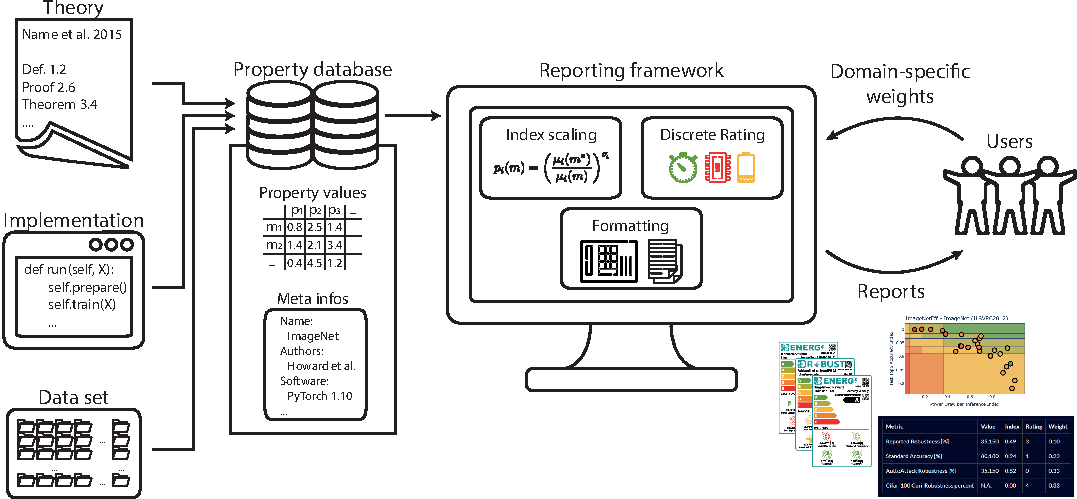
\includegraphics[width=.9\textwidth]{fig/framework.pdf}
    \caption{Schematic visualization of STREP, our proposed sustainable and trustworthy reporting framework. Internally, it processes databases of reported properties, which stem from applying implemented ML methods to specific data sets. Users can interact with the framework to gain an understanding of model properties in terms of their own priorities. Resource trade-offs are explicitly considered, and results can be represented more abstractly for audiences with limited ML knowledge.}
    \label{fig:framework}
\end{figure*}






\section{Current State of ML Reporting}
\label{sec:rw}

Reporting plays a vital role for bridging communication gaps between ML experts and less informed practitioners \cite{piorkowski_how_2021}.
The EU AI act \cite{eu_ai_hleg_assessment_2020} was manifested to ensure that ML is used in trustworthy \cite{chatila_trustworthy_2021,avin_filling_2021}, accountable \cite{hauer_overview_2023}, and responsible \cite{baum2022responsibility,Dignum/2019a} ways, and demands these systems to be designed safe, transparent, traceable, non-discriminatory, and environmentally friendly \cite{parliament_step_2023}.
The last aspect is especially noteworthy, as modern ML can act as a tool for making the world more sustainable \cite{van_wynsberghe_sustainable_2021,kar_how_2022}, but has also been shown to significantly impact our climate \cite{strubell_energy_2020,bender_dangers_2021,patterson_carbon_2021}.
Many works have put forward to investigate resource efficiency explicitly \cite{Assessing_Energy_Efficiency_of_ML,lacoste_quantifying_2019}, as resource consumption was found to be generally underreported \cite{Schwartz/etal/2020b,castano_exploring_2023}.
The works above underline that the current paradigm of ML reporting needs further improvement.
We start our contribution to the cause by characterizing the present state -- our assessment is summarized in \Cref{tab:reporting_overview}.

\setlength{\tabcolsep}{3pt}
\begin{table}
    \caption{Established reporting approaches and their drawbacks}
    \label{tab:reporting_overview}
    \centering
    \begin{tabular}{c|ccccc}
        Reporting & Sustainable & Interactive & Comprehensible & Usable & Reproducible \\
        \toprule
        Individual & & & & & \\
        Regular papers & \xmark$^\ast$ & \xmark & \xmark & \xmark$^{\times}$ & \ymark$^{\pitchfork}$ \\
        Model summaries & \multirow{2}{*}{\xmark$^\ast$} & \multirow{2}{*}{\xmark} & \multirow{2}{*}{\xmark$^\ast$} & \multirow{2}{*}{\xmark$^{\times}$} & \multirow{2}{*}{\xmark} \\
        (e.g., \cite{Mitchell/etal/2019a,arnold2019factsheets}) & & & & & \\
        Labels \cite{yeswecare,Assessing_Energy_Efficiency_of_ML} & \cmark & \xmark & \cmark & \ymark$^{\sqcap}$ & \ymark$^{\pitchfork}$ \\
        \midrule
        Benchmarks & \multirow{2}{*}{\xmark$^\ast$} & \multirow{2}{*}{\ymark$^{\diamond}$} & \multirow{2}{*}{\xmark} & \multirow{2}{*}{\cmark$^{\Join}$} & \multirow{2}{*}{\ymark$^{\pitchfork}$} \\
        (e.g., \cite{godahewa2021monash,croce2020robustbench,srivastava_beyond_2022}) & & & & & \\
        \midrule
        Databases & \multirow{2}{*}{\xmark$^{\ast}$} & \multirow{2}{*}{\ymark$^{\diamond}$} & \multirow{2}{*}{\xmark} & \multirow{2}{*}{\cmark$^{\Join}$} & \multirow{2}{*}{\ymark$^{\pitchfork}$} \\
        (e.g., \cite{paperswithcode,vanschoren2014openml}) & & & & & \\
        \midrule
        Our framework & \cmark & \cmark & \cmark & \cmark$^{\Join}$ & \ymark$^{\pitchfork}$ \\
        \bottomrule
        \multicolumn{6}{l}{$^{\ast}$  not explicitly considered to be important, only occasionally reported} \\
        \multicolumn{6}{l}{$^{\diamond}$  results can be sorted based on single reported properties} \\
        \multicolumn{6}{l}{$^{\times}$  not automated, need to be manually assembled} \\
        \multicolumn{6}{l}{$^{\sqcap}$  automated generation only limitedly supported} \\
        \multicolumn{6}{l}{$^{\Join}$  structural inconsistencies (e.g., properties not well-characterized)} \\
        \multicolumn{6}{l}{$^\pitchfork$  considered, but no guarantee that results can be exactly reproduced} \\
    \end{tabular}
\end{table}

Our literature review found that ML reporting generally takes place on one of three levels:
The first informs on properties of an \emph{individual} method or model, which in the most naive case, can be described in a scientific paper.
To allow for faster comparison and understanding, fact sheets \cite{arnold2019factsheets} and model cards \cite{Mitchell/etal/2019a} were proposed as higher-level summaries.
This idea is for example successfully implemented in the Hugging Face repository \cite{jain_hugging_2022}.
As these representations are still too technical to be understood by non-experts, the idea for establishing care labels \cite{yeswecare}, a more abstract and \emph{comprehensible} form of communication, was put forward.
In the context of \emph{sustainability}, this idea was adapted for reporting on ML resource efficiency more comprehensibly \cite{Assessing_Energy_Efficiency_of_ML} (in analogy to the EU energy labels \cite{eu-washingmachines}).
A central drawback of frameworks for individual reporting lies in their non-interactiveness -- their results cannot be customized to users' interests.
Consider a practitioner wanting to learn about a model's suitability for his specific use case and priorities, which might for example be subject to certain resource constraints.
In this case, the option of interactively controlling the importance of single model properties would help to align the framework's output with his needs.
Interacting with any system has also been shown to increase users' understanding and trust \cite{beckhsok}, which are desirable attributes for reporting frameworks.
In addition, most aforementioned works \cite{arnold2019factsheets,Mitchell/etal/2019a} also do not offer any automation for generating reports, which strongly impacts the \emph{usability} for experts wanting to report novel results.

\emph{Benchmarks} form the second level of reporting and summarize many individual reports for giving an overview of specific ML application domains.
These days, competitive leaderboards allow to compare the performance of SOTA methods in domains such as robustness testing \cite{croce2020robustbench}, time series forecasting \cite{godahewa2021monash}, language understanding \cite{srivastava_beyond_2022,wang_superglue_2019}, and commonsense reasoning \cite{sakaguchi_winogrande_2021}.
Several works assembled such benchmarks to investigate the performance of different methods across multiple data sets \cite{demsar_statistical_2006,ismail-fawaz_approach_2023}.
Cross-domain \emph{databases} are located on the third level and take the idea of benchmarks a step further, basically comprising different leaderboards across a wide range of domains.
Thanks to their open nature and direct coding interfaces, representatives like Papers With Code \cite{paperswithcode} and OpenML \cite{vanschoren2014openml} became highly popular.
As they offer direct access to data, methods, and training configurations  \cite{feurer_openml-python_2021}, these platforms are highly beneficial for new practitioners.
Model and data set repositories \cite{jain_hugging_2022} as well as platforms for performing ML experiments in an accelerated and unified way \cite{zaharia_accelerating_2018,demsar_orange_2013,Mierswa/etal/2006a} help in assembling such databases, and are sometimes directly integrated via interfaces.
Recent investigation suggests that promoting scientific papers and code via such platforms \cite{paperswithcode} helps in distributing research and achieving more citations \cite{kang_papers_2023}.

Opposed to individual reporting, these platforms offer limited means for interaction, as users can sort results based on their preference \cite{croce2020robustbench,vanschoren2014openml} or configure custom plots \cite{vanschoren2014openml,paperswithcode}.
More advanced mechanisms, like controlling the impact of different properties for the overall method rating, are unfortunately missing.
The comprehensibility and thus benefit for non-experts is questionable, as fundamental information on metrics and methods is only partially provided and high-level representations of individual results (e.g., via labels \cite{yeswecare}) are not offered.
As anyone can easily edit open databases, their usability is slightly impacted by the inconsistent reporting of properties.
As a small teaser to \Cref{sec:experiments}, we found many leaderboards to be only sparsely populated and specific properties being redundantly duplicated thanks to different spellings (e.g., ``params'' and ``parameters'').
Another big drawback of all mentioned reporting frameworks lies in their neglect of \emph{sustainability}.
Reporting on computing environment or consumed resources is only optional and not specifically motivated, and we later show further evidence that, as a result, many reported benchmarks are overly focused on predictive capabilities \cite{Schwartz/etal/2020b}.
Lastly, we want to also explicitly mention the problem of \emph{reproducibility} \cite{hutson_artificial_2018,pineau_improving_2021}, which is of utmost importance in the context of trustworthiness.
Established frameworks support linking code \cite{paperswithcode} and offer interfaces to selected ML libraries \cite{vanschoren2014openml}, but ultimately, they do not test whether reported results can actually be reproduced.
Even with available code, information on the utilized hardware and software setup is usually not provided -- we argue that SOTA reporting should explicitly demand such information.

\Cref{tab:reporting_overview} lists our assessment of current reporting and its drawbacks at a glance.
We want to stress that we understand all established works to be highly important and successful contributions that we want to build on.
In the following section, we present STREP, our own take on sustainable and trustworthy reporting.
In comparison to the discussed approaches, we specifically designed our framework to be more
\emph{sustainable}, since we offer a holistic approach for reporting any method's resource trade-offs in its respective computational environment,
\emph{interactive}, since users can align the impact of each property for the overall assessment with their priorities, and more
\emph{comprehensible}, since we directly offer means for generating high-level labels.
As motivated earlier, the latter two aspects are directly linked to the trustworthiness of any system.
In terms of usability and reproducibility aspects, we are aware of their importance but do not push improvements with this work.
We still deem STREP to be highly usable -- it can be easily used to investigate any given database and generate different report representations automatically.
However, it does neither tackle the aforementioned inconsistencies in open databases nor the limited reproducibility, as both issues boil down to how well-organized and -documented the original reported results are.










\section{STREP - Sustainable and Trustworthy Reporting}

To make reporting more sustainable and trustworthy, we devised central questions that address the identified flaws and need to be explicitly considered:
(Q1) How can reported method properties be characterized in a resource-aware way?
(Q2) How can the practical computing environment be taken into account?
(Q3) What means for interactive investigation can be offered?
(Q4) How can users at different levels of ML understanding be informed?
This section is structured accordingly, and our proposed STREP framework implements possible answers to Q1--Q4.

\subsection{Characterizing ML Properties}
\label{sec:meth:characterizing}

Good reporting requires to first thoroughly characterize the nature of ML experiments and properties that methods may exhibit.
While other works have addressed this challenge \cite{Assessing_Energy_Efficiency_of_ML,yeswecare}, STREP uses a characterization that is better suited for practical use.
Therefore, we mostly align it along established terminology \cite{paperswithcode}, for which thousands of reported \emph{evaluations} can already be found online.

\begin{definition}\label{def:evaluation}
Any evaluation is defined by the tuple $(d, t, m)$, which represents:
\begin{enumerate*}[label=(\roman*)]
    \item a data set $d$,
    \item a task type $t$, i.e., an abstract action to be performed on $d$, and
    \item a ML method $m$, that can practically perform this action.
\end{enumerate*}
The theoretical space of all possible evaluations $(d, t, m)$ is denoted by $\mathcal{D}\times\mathcal{T}\times\mathcal{M}$; however, certain combinations might be inadmissible.
\end{definition}

Concisely, an evaluation $(d, t, m)$ represents the abstraction of using a specific method $m$ to solve a particular task $t$ on given data $d$.
An example would be to classify ($t$) a fixed number of ImageNet images ($d$) with MobileNetV2 ($m$) \cite{howard_mobilenets_2017}.
Evaluations already encompass respective hyperparameters (e.g., optimizer configuration, preprocessing, \dots), which might have a strong impact on practical performance.
For the sake of clarity, we do not explicitly denote them in our characterization, but want to emphasize the need for reporting them in detail -- to give a good example, OpenML's database distinguishes between different method \emph{setups} \cite{vanschoren2014openml}.
As indicated by the last sentence in \Cref{def:evaluation}, fixing any $d$, $t$, or $m$ potentially limits the other options, as for example image classification cannot be performed on time series data.
It is essential to differentiate between tasks (training, inference, architecture search, \dots), as each task has its own quantities for assessing the performance:

\begin{definition}\label{def:properties}
Any combination of data $d$ and task $t$ determines a space of properties $\bm{p}(d, t) = \{p_{(d, t)}(m)\} \subset \mathbb{R}^n$ in which methods $m$ score via property functions $p_{(d, t)_i}: \mathcal{M} \rightarrow \mathbb{R}$ for $1 \leq i \leq n$. A specific evaluation result $\bm{p}_{(d, t)}(m)$ thus is a $n$-dimensional vector of properties that $m$ exhibits when being applied to perform $t$ on $d$.
\end{definition}

Note that where other works refer to this as \emph{metrics} \cite{paperswithcode} or \emph{measures} \cite{vanschoren2014openml}, we instead chose to report \emph{properties} in STREP, whose denotion $p$ is easier to formally distinct from the method choice $m$.
We want to stress that $\mathcal{P}$ only represents measurable, numeric properties like accuracy or running time, to stay with the ImageNet example above.
Obviously, some additional information also needs to be reported -- these \emph{meta properties} might be textual descriptions, related literature, or implementation details, to name but a few.
While they play an important role for comprehensibility and reproducibility, we do not formally denote them, as they are irrelevant for the numerical comparison of methods.
In practice, different properties and dimensions of $\mathcal{P}$ can be grouped into either describing predictive quality (error, accuracy, \dots) or resource usage (running time, model size, \dots). 
Usually, we expect these two groups to compete, as deploying ML efficiently requires to investigate the trade-off between predictive capabilities and resource demand \cite{Assessing_Energy_Efficiency_of_ML}.
As such, we support others in their argumentation that explicitly reporting on properties in both groups is mandatory for sustainable ML development \cite{Schwartz/etal/2020b}.
Opposed to the discussed established frameworks (recall \Cref{sec:rw}), STREP gives clear incentives to do so (e.g., via error messages when no resource-allied properties are reported).
% Also consider that properties might also be traded across different tasks.
% For example, it has become common practice to specifically focus on efficient deployment of models \cite{buschjager2017decision}, and even consider this during training \cite{howard_mobilenets_2017}.

\subsection{Taking Execution Environments Into Account}
\label{sec:meth:comparability_and_index_scale}

In practice, properties exhibited by a method are subject to the real-world hardware and software used for performing the evaluation.
Even though some methods possess certain theoretical (i.e., static \cite{yeswecare}) attributes, it is not guaranteed that they hold in practice (e.g., due to coding mistakes \cite{sun_empirical_2017}).
Unfortunately, we find that most established benchmarks neglect the importance of this computational \emph{environment}, which is why we explicitly consider it in STREP.
We extend the definitions above accordingly:

\begin{definition}\label{environment}
Any evaluation $(d, t, e)$ is executed in an \emph{environment} $e \in \mathcal{E}$, which is defined by the choice of hardware and software. As they impact how any method performs in practice, we adjust \Cref{def:properties} accordingly: $\bm{p}_{(d, t, e)} = \{p_{(d, t, e)_i}: \mathcal{M} \times \mathcal{E} \rightarrow \mathbb{R} \}$ is now also subject to $e$.
\end{definition}

In addition to earlier restrictions, we may find that environments impose further limitations (and vice-versa).
As examples, consider SOTA deep learning models that demand several gigabytes of memory capacity \cite{strubell_energy_2020}, or the the limited range of readily usable methods for edge \cite{buschjager2020site} or quantum hardware \cite{mucke2023feature}.
For improved readability, we from now on omit the underlying data, task, and environment choice $(d, t, e)$ and resort to simply denoting method properties as $\bm{p}(m) = \{p_i(m)\}$.
From the diversity of environments (e.g., desktops, laptops, compute clusters, embedded devices), a new problem arises:
The measurements of resource-allied properties like running time can scale with multiple levels of magnitude when running a fixed evaluation in different environments.
While the impact on resource demand is most obvious, it could even happen that predictions change with the environment, e.g., due to algorithmic changes across library versions.
In order to compare properties, even across multiple environments, STREP therefore adapts relative \emph{index scaling} \cite{Assessing_Energy_Efficiency_of_ML}:

\begin{equation}\label{eq:index}
    p_i(m)=\left(\frac{\mu_i(m^*)}{\mu_i(m)}\right)^{\sigma_i}=\left(\frac{ (\min_{m'\in \mathcal{M}} \mu_i(m')^{\sigma_i})^{\sigma_i}}{\mu_i(m)}\right)^{\sigma_i},
\end{equation}

Where the original work calculates index values $p_i(m)$ based on global references, we instead propose to relate the real measurements $\mu_i(m)$ to the empirically best-performing method $m^\ast$ on the $i$-th property.
We deem this approach advantageous to global referencing since it neatly solves the problem of choosing good references.
With \Cref{eq:index}, the property values $p_{i}$ become bounded by the interval $(0, 1]$ and describe the behavior in the given environment relatively; the higher the value, the closer it is to the best empiric result which receives $p_i(m^*) = 1$.
On the index scale, properties are more easily comparable -- a value of $0.6$ always indicates that the method achieves 60\% of the best empirically known result, regardless of which property is discussed.
Index scaling also neatly solves another problem -- most properties (e.g., running time and power draw) require minimization for improvement, but some exceptions (e.g., accuracy) demand maximization.
To handle this issue, the constant $\sigma_i$ is introduced and denotes whether the corresponding $i$-th property should be maximized ($\sigma_i=-1$) or minimized ($\sigma_i=+1$).
As given in \Cref{eq:index}, it flips certain scales and the understanding of best-performing reference (i.e., highest or lowest value).
When measured properties and additional information via meta properties are provided to STREP, it automatically computes the environment-specific index values (and updates them if new best scores are added).

\subsection{Offering Means for Interaction}
\label{sec:meth:customization_via_weighting}
While methods should generally perform well across all properties, there can also be use cases where certain aspects are more important.
To give some examples, consider safety-critical applications that demand highly robust predictions \cite{croce2020robustbench}, or embedded systems with tight memory constraints \cite{buschjager2020site}.
Unfortunately, as listed in \Cref{tab:reporting_overview}, established systems only support interactions to a certain degree.
STREP assesses any method's suitability for a given task and data under consideration of the practitioner's priorities via a \emph{weighted compound performance score}:

\begin{equation}\label{eq:compound}
P(m) = \sum_{i=1}^n w_i p_i(m) \textrm{ with } \forall i, w_i\geq0  \textrm{ and }  \sum_{i=1}^k w_i=1
\end{equation}

Normalizing the weights $w_i$ assures that the compound score is also bounded by $(0, 1]$, with $P(m)=1$ indicating the unlikely case that $m$ achieves the best possible results across all reported properties.
With property grouping as introduced in \Cref{sec:meth:characterizing}, users are enabled to control the importance of resource efficiency.
In an extreme setting, resource-allied properties can be disregarded by setting their weight to zero.
Likewise, users can purely concentrate on a method's compute demand and leave out all non-resource properties.
To generally achieve good trades, STREP per default assigns weights such that both groups are equally impactful in \Cref{eq:compound}.

Another opportunity for making the reporting framework more interactive lies in the representation of results.
Like other frameworks, STREP provides plain textual descriptions, numeric tables, and plots that display reported data more visually and intuitively \cite{cui_visual_2019}.
Via its interactive interface \cite{dabbas_interactive_2021}, users can explore the reported results and also switch between and thus understand the real measurement and relative index scales.
Lastly, STREP also interactively displays individual results in a more comprehensible representation.

\subsection{Informing on Different Levels of Understanding}
\label{sec:meth:automated_labeling}

While experts from the field can investigate in-depth tables and plots, many works have put forward to establish more comprehensible means of reporting \cite{yeswecare}.
We support this call and formulate several ideas for implementing this practically.
First of all, properties can be represented with the help of intuitive badges \cite{yeswecare} to express their underlying meaning metaphorically.
To make numeric values comprehensible, we can subdivide each index scale into bins and color-code the performance along each property \cite{Assessing_Energy_Efficiency_of_ML}.
Naturally, each label should also report the evaluation setting (task, data, environment, method) via text, badges, or logos.
In-depth information and additional material can be easily embedded via QR codes.
To make the label representation feasible, it is key to automatically generate these abstract summaries, as opposed to manual compilation \cite{arnold2019factsheets,Mitchell/etal/2019a}.
For this reason, STREP features a fully automated label generator that puts all suggested ideas into effect.

















\section{Experimental Evaluation}
\label{sec:experiments}

\begin{figure}
    \centering
    \includegraphics[width=.9\textwidth]{fig/ui.png}
    \caption{User interface of our STREP software. It depicts the trade-offs among properties, automatically generates a tabular and label representation of any method's performance (upon hovering over single points) and allows for interaction via controlling the weights and customizing the plots.}
    \label{fig:ui}
\end{figure}

\setlength{\tabcolsep}{3pt}
\begin{table}
    \caption{Established reporting approaches and their drawbacks}
    \label{tab:databases}
    \centering
    \begin{tabular}{lccccccc}
        \toprule 
        Database & ImageNetEff & RobustBench & Forecasting & Papers With Code \\
        \midrule
        Data sets & 1 & 3 & 114 & 161 \\
        Tasks & 2 & 1 & 1 & 120 \\
        Methods & 31 & 150 & 11 & 3830 \\
        Environments & 8 & 1 & 1 & 1 \\
        Properties (resources) & 9 (4) & 7 (0) & 9 (4) & 495 (10) \\
        Evaluations & 232 & 207 & 1254 & 4760 \\
        Incompleteness &  4.34 \% & 31.03 \% &  0.00 \% & 19.70 \% \\
        \bottomrule
    \end{tabular}
\end{table}

\begin{figure}
    \centering
    \begin{minipage}[t]{.48\textwidth}
        \includegraphics[width=\textwidth]{fig/pwc_stats.pdf}
        \caption{Papers With Code is only sparsely populated, with only few data reported for thousands of (data $\times$ task) combinations.}
        \label{fig:pwc_stats}
    \end{minipage}
    \hfill
    \begin{minipage}[t]{.48\textwidth}
        \includegraphics[width=\textwidth]{fig/db_filtered.pdf}
        \caption{Filtering steps applied to the sparse database of Papers With Code for identifying interesting benchmarks for our investigations.}
        \label{fig:db_filtered}
    \end{minipage}
\end{figure}

We now demonstrate what insights the introduced ideas provide in practice by investigating established report databases with the help of our STREP software. 

\subsection{Experiment Setup}
Our Python library (available at \url{github.com/raphischer/strep}) handles property databases via \texttt{pandas} \cite{jeff_reback_2022_6053272} dynamically reports tables, interactive plots, and labels via \texttt{Plotly} and \texttt{Dash} \cite{dabbas_interactive_2021}.
The user interface is displayed in \Cref{fig:ui} -- users can bring their own custom property databases or explore four readily processed databases:
(1) reported efficiency of ImageNet models across multiple environments \cite{Assessing_Energy_Efficiency_of_ML}, (2) the RobustBench leaderboard \cite{croce2020robustbench}, (3) results from forecasting Monash time series \cite{godahewa2021monash} with deep neural networks, and (4) a extract from Papers With Code \cite{paperswithcode}.
Following our characterization as proposed in \Cref{sec:meth:characterizing}, we provide the database statistics in \Cref{tab:databases}.
They list total numbers across all task $\times$ data combinations, which each determine the applicable properties and methods.
As shown in \Cref{fig:pwc_stats}, Papers With Code is only sparsely populated, with few evaluations and properties reported for most cases (i.e., data $\times$ task combinations).
For this reason, we identified the most interesting benchmarks via filtering steps described in \Cref{fig:db_filtered}.
With \emph{Incompleteness}, we denote the average amount of \texttt{NAN} values found in the evaluations of each data $\times$ task combination.
The weights were chosen such that each property group (resources or predictive quality) is equally impactful for \Cref{eq:compound} -- the properties within each group are also equally weighted.
The ``most important'' properties discussed later on were chosen heuristically, as the ones with highest number of reported values.
The Papers With Code and RobustBench databases can be re-created with our linked code while the other two were pre-assembled (further information provided in the respective literature).
Following the call for openly reporting any paper's environmental impact \cite{Schwartz/etal/2020b}, we estimate the total carbon emissions of this work to about 6 CO$_2$e -- four full work weeks of running a CPU-only laptop \cite{lacoste_quantifying_2019} for software development and writing.
We invite readers to also use our STREP application for exploring the databases in detail, as this paper is limited to investigating exemplary results.

\begin{figure*}
    \centering
    \includegraphics[width=.49\textwidth]{fig/scatter_ImageNetEff.pdf}
    \includegraphics[width=.49\textwidth]{fig/scatter_RobustBench.pdf}
    \\
    \vspace{1em}
    \includegraphics[width=.49\textwidth]{fig/scatter_Forecasting.pdf}
    \includegraphics[width=.49\textwidth]{fig/scatter_Papers With Code.pdf}
    \caption{Property trade-offs of different methods on selected data. Node colors indicate the compound score across all property dimensions, from which the two most important ones are shown as axes.}
    \label{fig:prop_spaces}
\end{figure*}    

\subsection{Trade-offs and Correlation of Properties}

We start by investigating the relations between important reported properties.
For four selected data sets (one from each databases), we display two-dimensional scatter plots in \Cref{fig:prop_spaces}.
Due to using the index scale from \Cref{eq:index}, all values are bounded and improving any property corresponds to a higher score.
In cases where properties are not reported (i.e., \texttt{NAN} value in the data frame), we assign $p_i(m) = 0$.
The node colors indicate the compound score over all properties, as introduced in \Cref{eq:compound}.
We see that the ImageNet models seem to be scattered along a multi-dimensional Pareto-front, with the two shown axes clearly trading against each other.
For RobustBench, on the other hand, the two displayed properties seem to be strongly correlated.
We display the complete properties of the best and worst options for each data set via star plots in \Cref{fig:prop_stars}.
They demonstrate how the proposed relative index scale can unify the reporting of multi-dimensional ML properties, despite their origin from very different domains and tasks.
Even though the axes describe totally different phenomena like running time, prediction errors, or model size, their index values remain easily comparable.
Where users of other reporting frameworks are restricted to sorting reports based on single properties, these STREP plots allow to explore the multi-dimensional relations between properties at an arbitrary depth.


\begin{figure*}
    \centering
    \includegraphics[width=.243\textwidth]{fig/true_best_ImageNetEff.pdf}
    \hfill
    \includegraphics[width=.243\textwidth]{fig/true_best_RobustBench.pdf}
    \hfill
    \includegraphics[width=.243\textwidth]{fig/true_best_Forecasting.pdf}
    \hfill
    \includegraphics[width=.243\textwidth]{fig/true_best_Papers With Code.pdf}
    \caption{All properties of the best and worst performing methods displayed via star plots on selected data. Due to the relative index scaling, all properties are equally bounded and easily comparable.}
    \label{fig:prop_stars}
\end{figure*}

\begin{figure}
    \centering
    \includegraphics[width=.95\textwidth]{fig/correlation_imagenet_fc.pdf}
    % \includegraphics[width=.48\textwidth]{fig/imagenet_correlation.pdf}
    % \hfill
    % \includegraphics[width=.48\textwidth]{fig/fc_correlation.pdf}
    \caption{Correlation between different properties in the ImageNet and Forecasting databases. As expected, certain characteristics like number of parameters and model file size are positively correlated, while trade-offs in terms of accuracy and resource usage are negatively correlated.}
    \label{fig:prop_corr_imagenet}
\end{figure}


With help of the Pearson correlation coefficient (PCC), we can numerically quantify trades in the form of pairwise property correlation.
Values near one, zero, or minus one respectively indicate strong correlation, no relation, or trades (i.e., negative correlation).
For the ImageNetEff and Forecasting data, this is displayed in \Cref{fig:prop_corr_imagenet}.
We find strong correlation between (1) model parameters and file size, (2) running time and power draw, as well as (3) accuracy and error properties.
The latter also tends to be un- or even negatively correlated with other properties, which indicates resource trade-offs.
This also supports our call for grouping and equally reporting properties for predictive capabilities and resource consumption.


\begin{figure*}
    \centering
    \includegraphics[width=\textwidth]{fig/prop_corr.pdf}
    \caption{Distributions of pairwise correlation between properties across all data sets and tasks. Index scaling is more suitable for comparing trade-offs, as these distributions have a more distinct, bimodal, and stretched out shape, and tend to entail either positive or negative correlation.}
    \label{fig:prop_corr}
\end{figure*}

\begin{figure}
    \centering
    \begin{minipage}[t]{.49\textwidth}
        \includegraphics[width=\textwidth]{fig/pwc_corr.pdf}
        \caption{Property correlations for Papers With Code tasks that also report on resource usage versus tasks that solely focus on prediction quality.}
        \label{fig:pwc_corr}
    \end{minipage}
    \hfill
    \begin{minipage}[t]{.49\textwidth}
        \includegraphics[width=\textwidth]{fig/pwc_comp_impact.pdf}
        \caption{Correlation of ranking methods based on a single property versus based on our compound score, which is aggregated from all properties.}
        \label{fig:pwc_comp_impact}
    \end{minipage}
\end{figure}

%TODO rewrite - first talk about their shapes, than compare index and value differences
% Investigating the PCCs across all properties also demonstrates the power of index scaling, as introduced in \Cref{sec:meth:comparability_and_index_scale}.
We show the distribution of PCCs across all databases and properties in \Cref{fig:prop_corr}, computed once for the original measurements and once for the scaled index values.
% Firstly, the index scaled results provide more spaced-out distributions of correlation.
% Some of them also have a more distinct bimodal shape, with the antimode being placed nearer to zero correlation.
% This indicates that with relative scaling, properties are more likely to be either negatively or positively correlated.
For the ImageNetEff and Forecasting data, we observe bimodal shapes, as already indicated in the more in-depth results from \Cref{fig:prop_corr_imagenet}.
On the other hand, the distributions for RobustBench and Papers With Code are heavily tilted towards high PCCs.
Index scaling seems to spread the distributions and make their shapes more distinct. 
We assume that the tilted shapes originate from reporting overly focused on predictive performance, which can already be seen in the vanishingly small number of resource properties in \Cref{tab:databases} -- on average, we found only 2\% of the reported properties in Papers With Code to fall into the resource category.
We test our assumption with \Cref{fig:pwc_corr}, where the database was split into evaluations that have at least some reported resource usage versus ones that solely focus on predictive quality.
The assessed PPC distributions for both groups clearly support our intuition -- the resource-aware distribution is much less tilted and features many correlations near zero.
This indicates that here interesting trades between different properties occur, under are under-reported for the other evaluations.

\subsection{Resource-aware and Comprehensible Scoring}

Next, we want to explore the effect of using our compound score (\Cref{eq:compound}) to assess overall method performance, under consideration of all reported properties and trades.
It is opposed to just concentrating on a single property, as it is the case with established frameworks that only allow for sorting (recall \Cref{tab:reporting_overview}).
We experimentally investigate this by assessing the rank correlation (Spearman's $\rho$) of sorting applicable methods for any task based on either (1) the most important property or (2) our compound score.
The resulting distribution of $\rho$ values across all databases is depicted in \Cref{fig:pwc_comp_impact}.
Firstly, it shows that on average both ranking approaches are positively correlated, which is to be expected -- the single property is also considered by the compound score.
The distributions of ImageNetEff and RobustBench are rather simple (only few benchmark rankings considered), but clearly demonstrate that considering all properties seems to strongly impact the understanding of ``good'' performance.
This is even more dramatically observed in the other databases, where some tasks and data sets even have low or negative correlation -- the ranking seems to completely change when all properties are taken into account.
On Papers With Code, which we already showed to be heavily biased towards optimizing predictive capabilities, we find the highest rank correlations.
However, even the average value of $\rho=0.75$ is not very high on the scale, and demonstrates the importance of considering all properties when assessing method performance.
We want to once more emphasize that our compound performance assessment is customizable -- we here use the heuristic weights explained earlier, but STREP allows users to interactively align the importance of properties with their priorities (e.g., to favor methods with low resource demand).

\begin{figure*}
    \centering
    \includegraphics[width=\textwidth]{fig/environment_changes.pdf}
    \caption{Impact of environment choice on ImageNet efficiency. The given compound scores are calculated from the environment-specific property index values. The vertical distance between model instances shows their performance stability across environment choice. }
    \label{fig:env_changes}
\end{figure*}

As explained in \Cref{sec:meth:comparability_and_index_scale}, both the compound score as well as single properties are subject to the execution environment in which the method is deployed.
For this reason, \Cref{fig:env_changes} investigates this effect in the ImageNetEff database.
The vertical distance between model points indicates how stable their efficiency is across different environments.
Models like MobileNetV2 \cite{howard_mobilenets_2017} seem to generally perform rather efficiently, whereas certain architectures like ResNets and VGG have very mixed compound performances.
These results are evidence that the environment greatly impacts method properties and thus should be explicitly reported.
RobustBench and Forecasting experiments were all performed on unified hardware -- it would be interesting to test how different environments might change the empiric behavior.
For Papers With Code, the environment is, in some cases, described in the associated paper.
However, it would be much more beneficial if this information was explicitly demanded whenever people report new results, ideally together with the very environment-specific compute utilization.

\begin{figure}
    \centering
    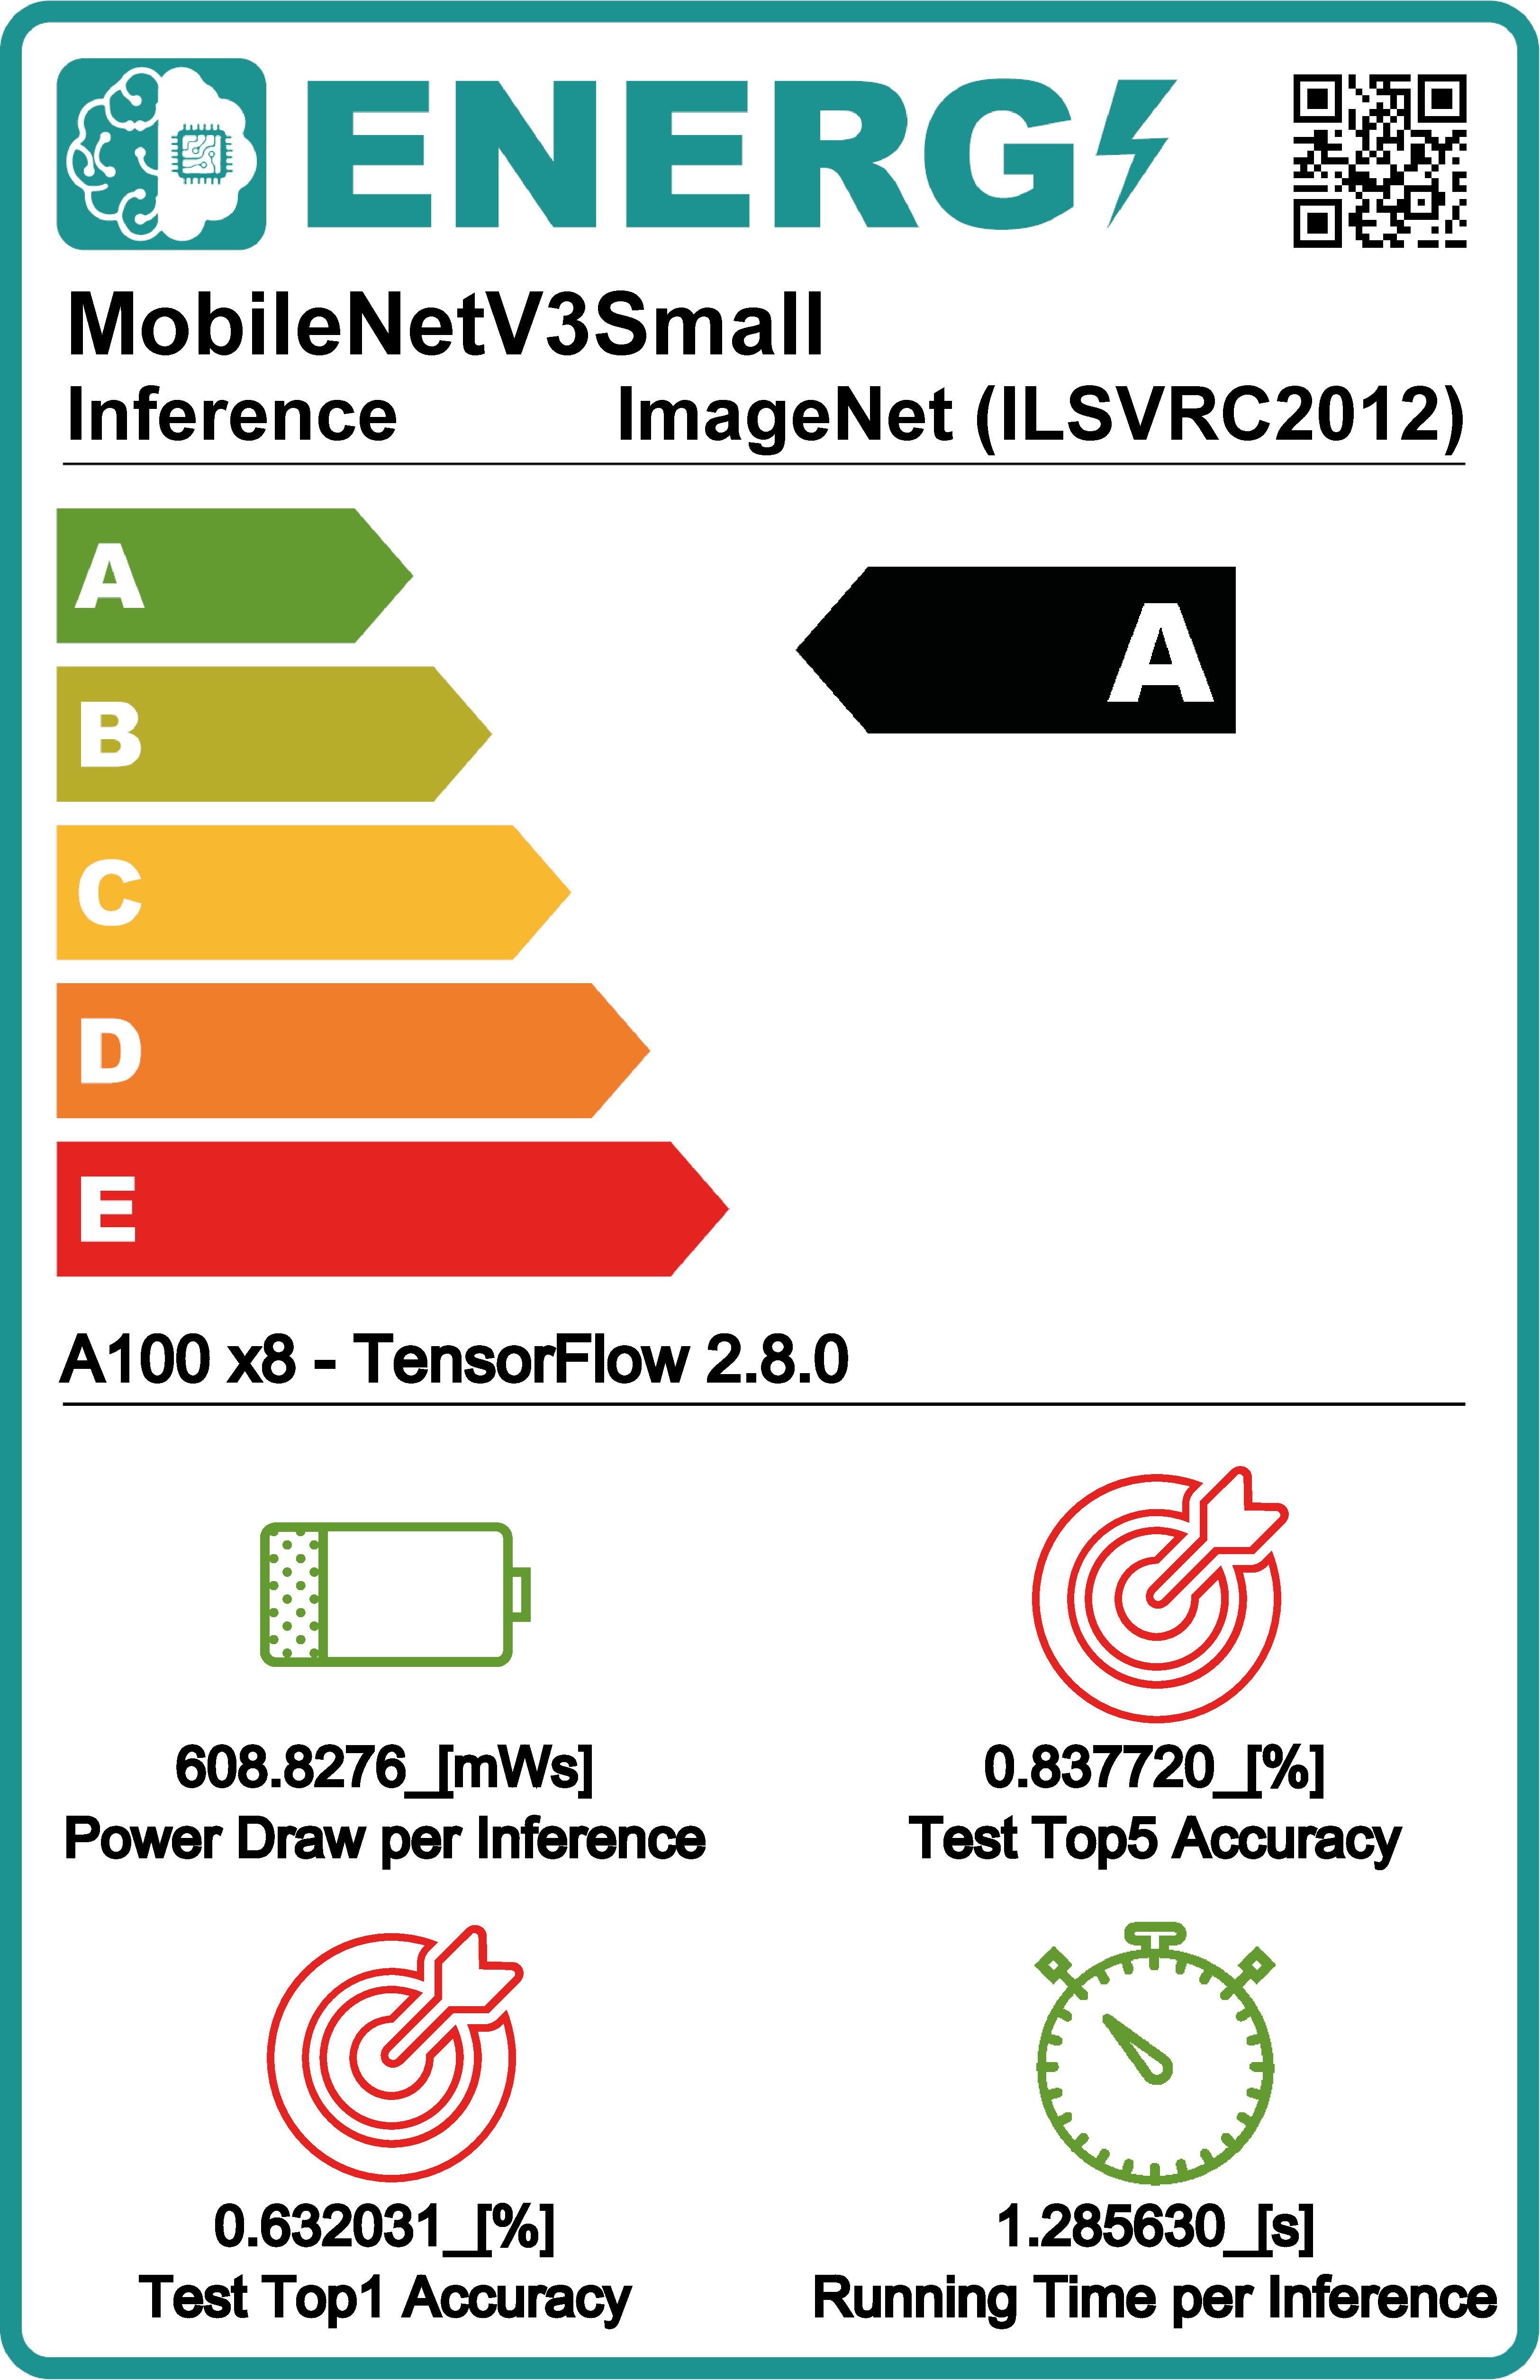
\includegraphics[width=.22\textwidth]{fig/energy_label_MobileNetV3Small_A100_x8_-_TensorFlow_2.8.0.pdf}
    \hfill
    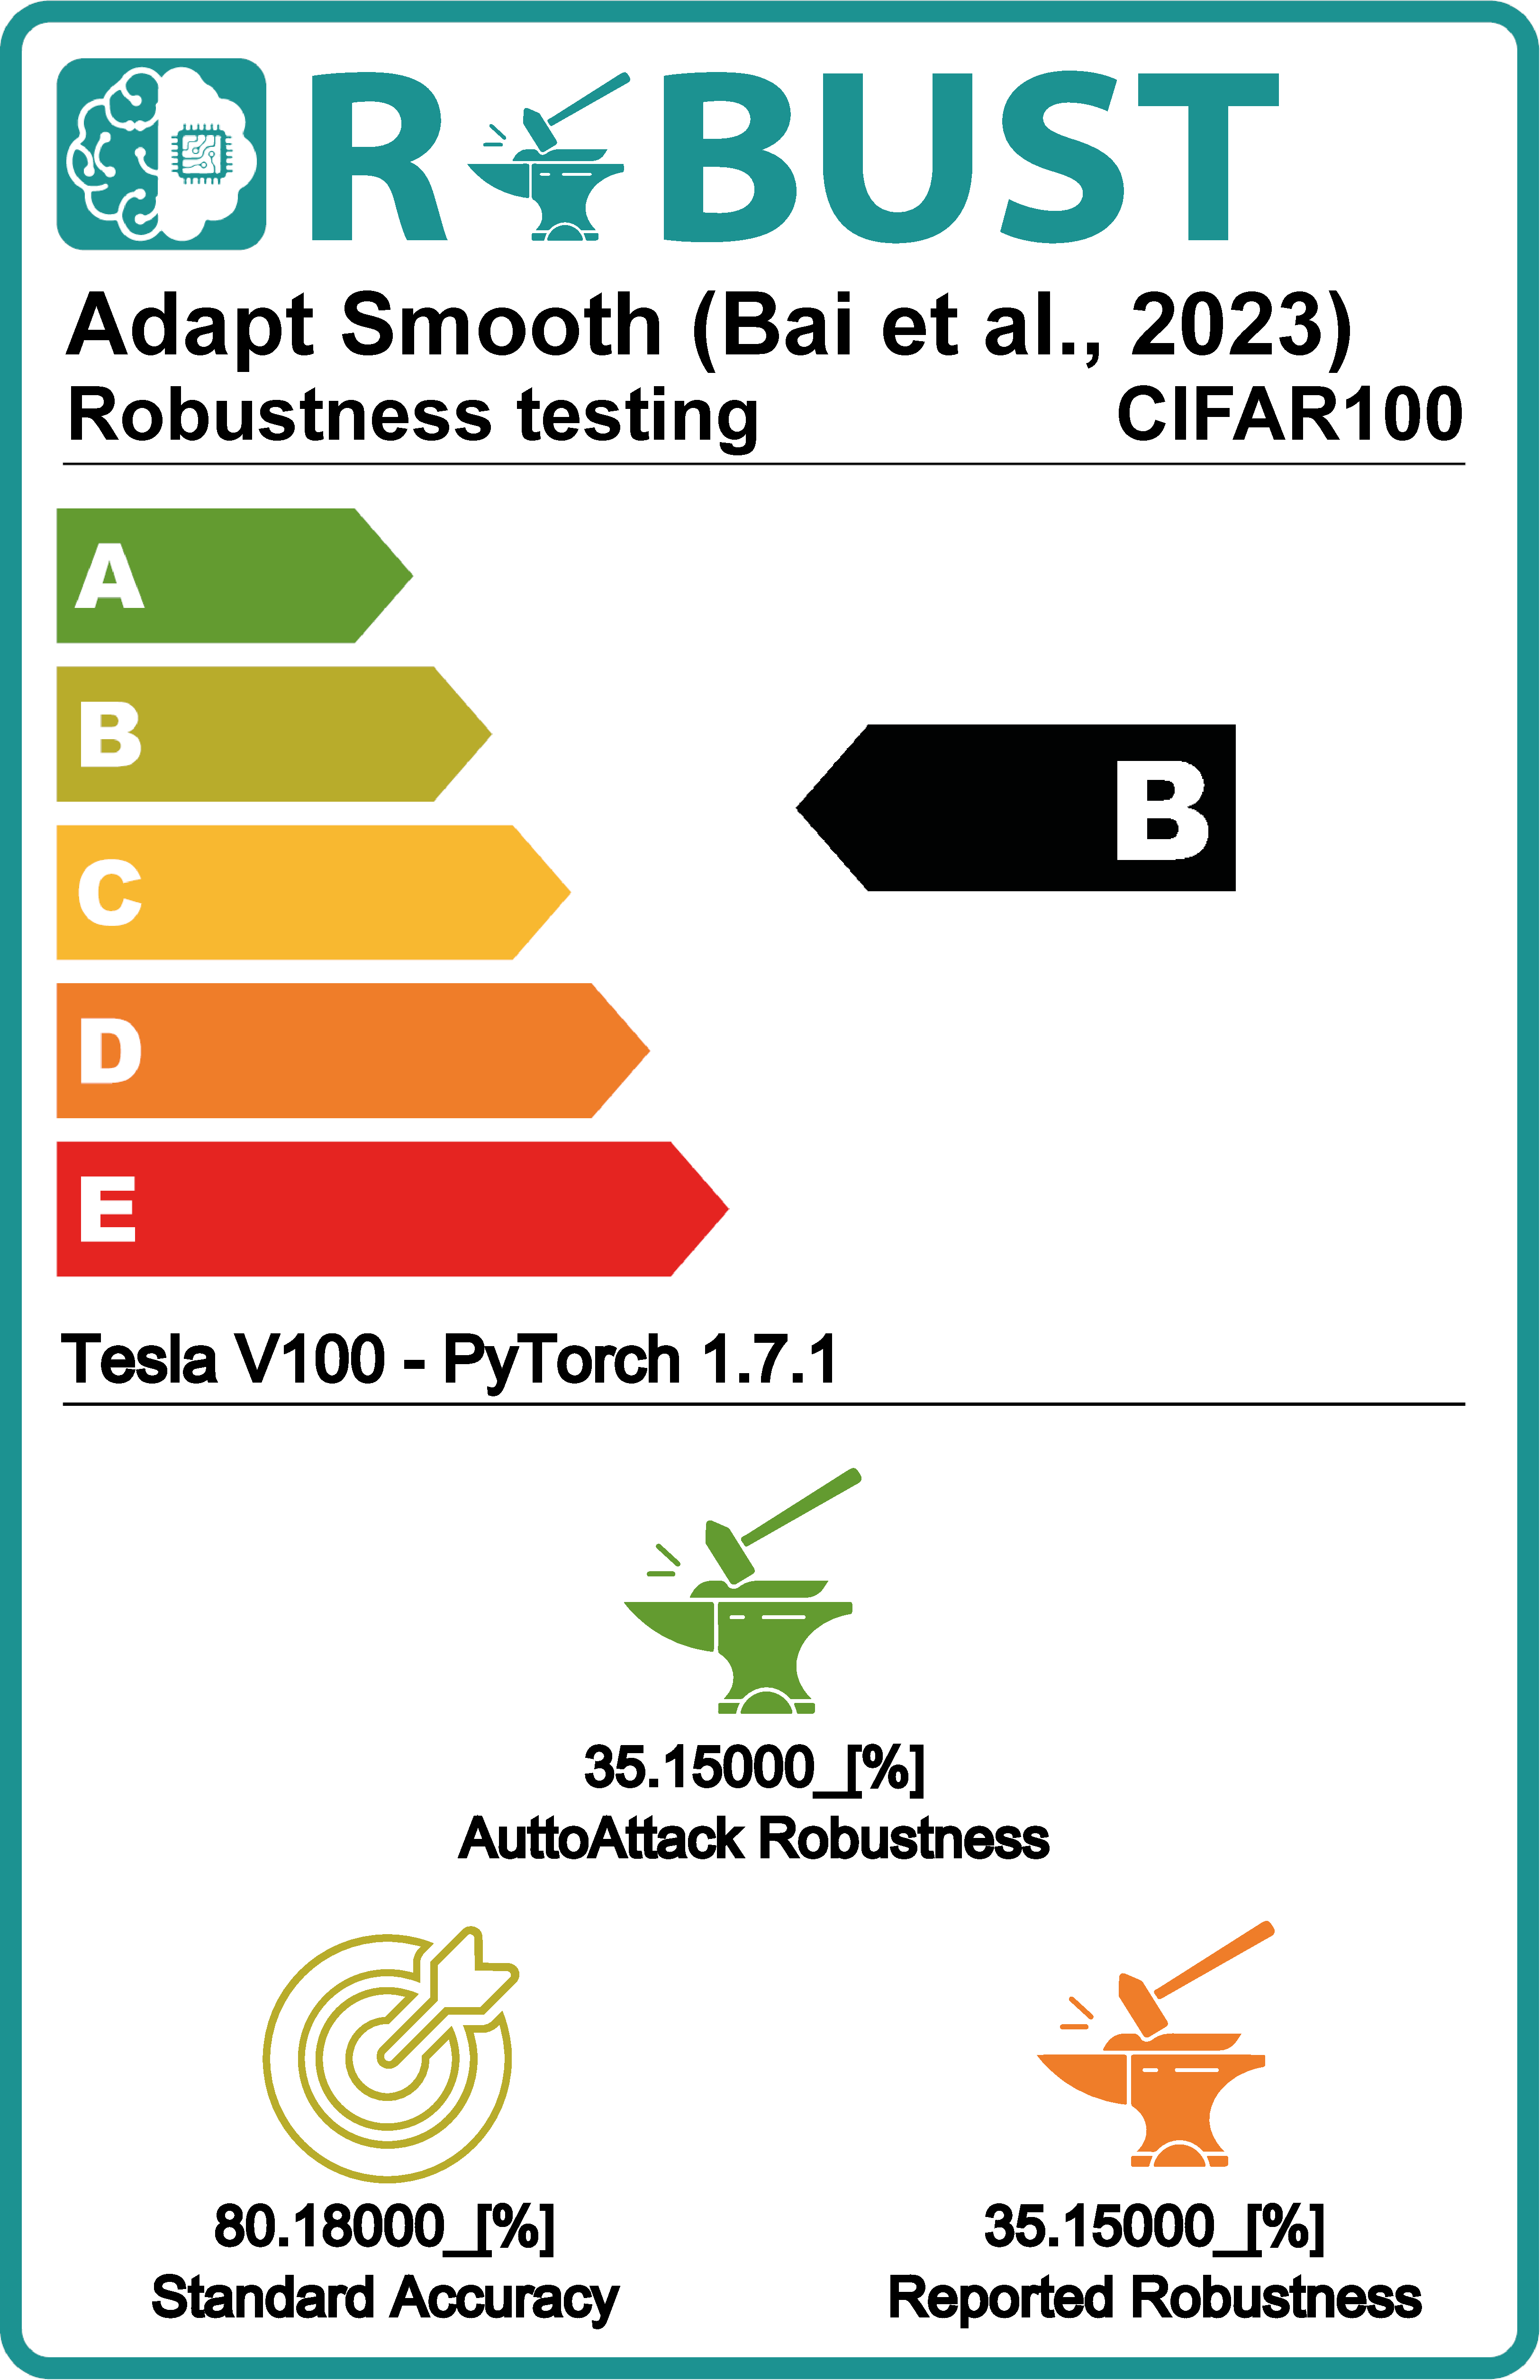
\includegraphics[width=.22\textwidth]{fig/energy_label_Bai2023Improving_trades_Tesla_V100_-_PyTorch_1.7.1.pdf}
    \hfill
    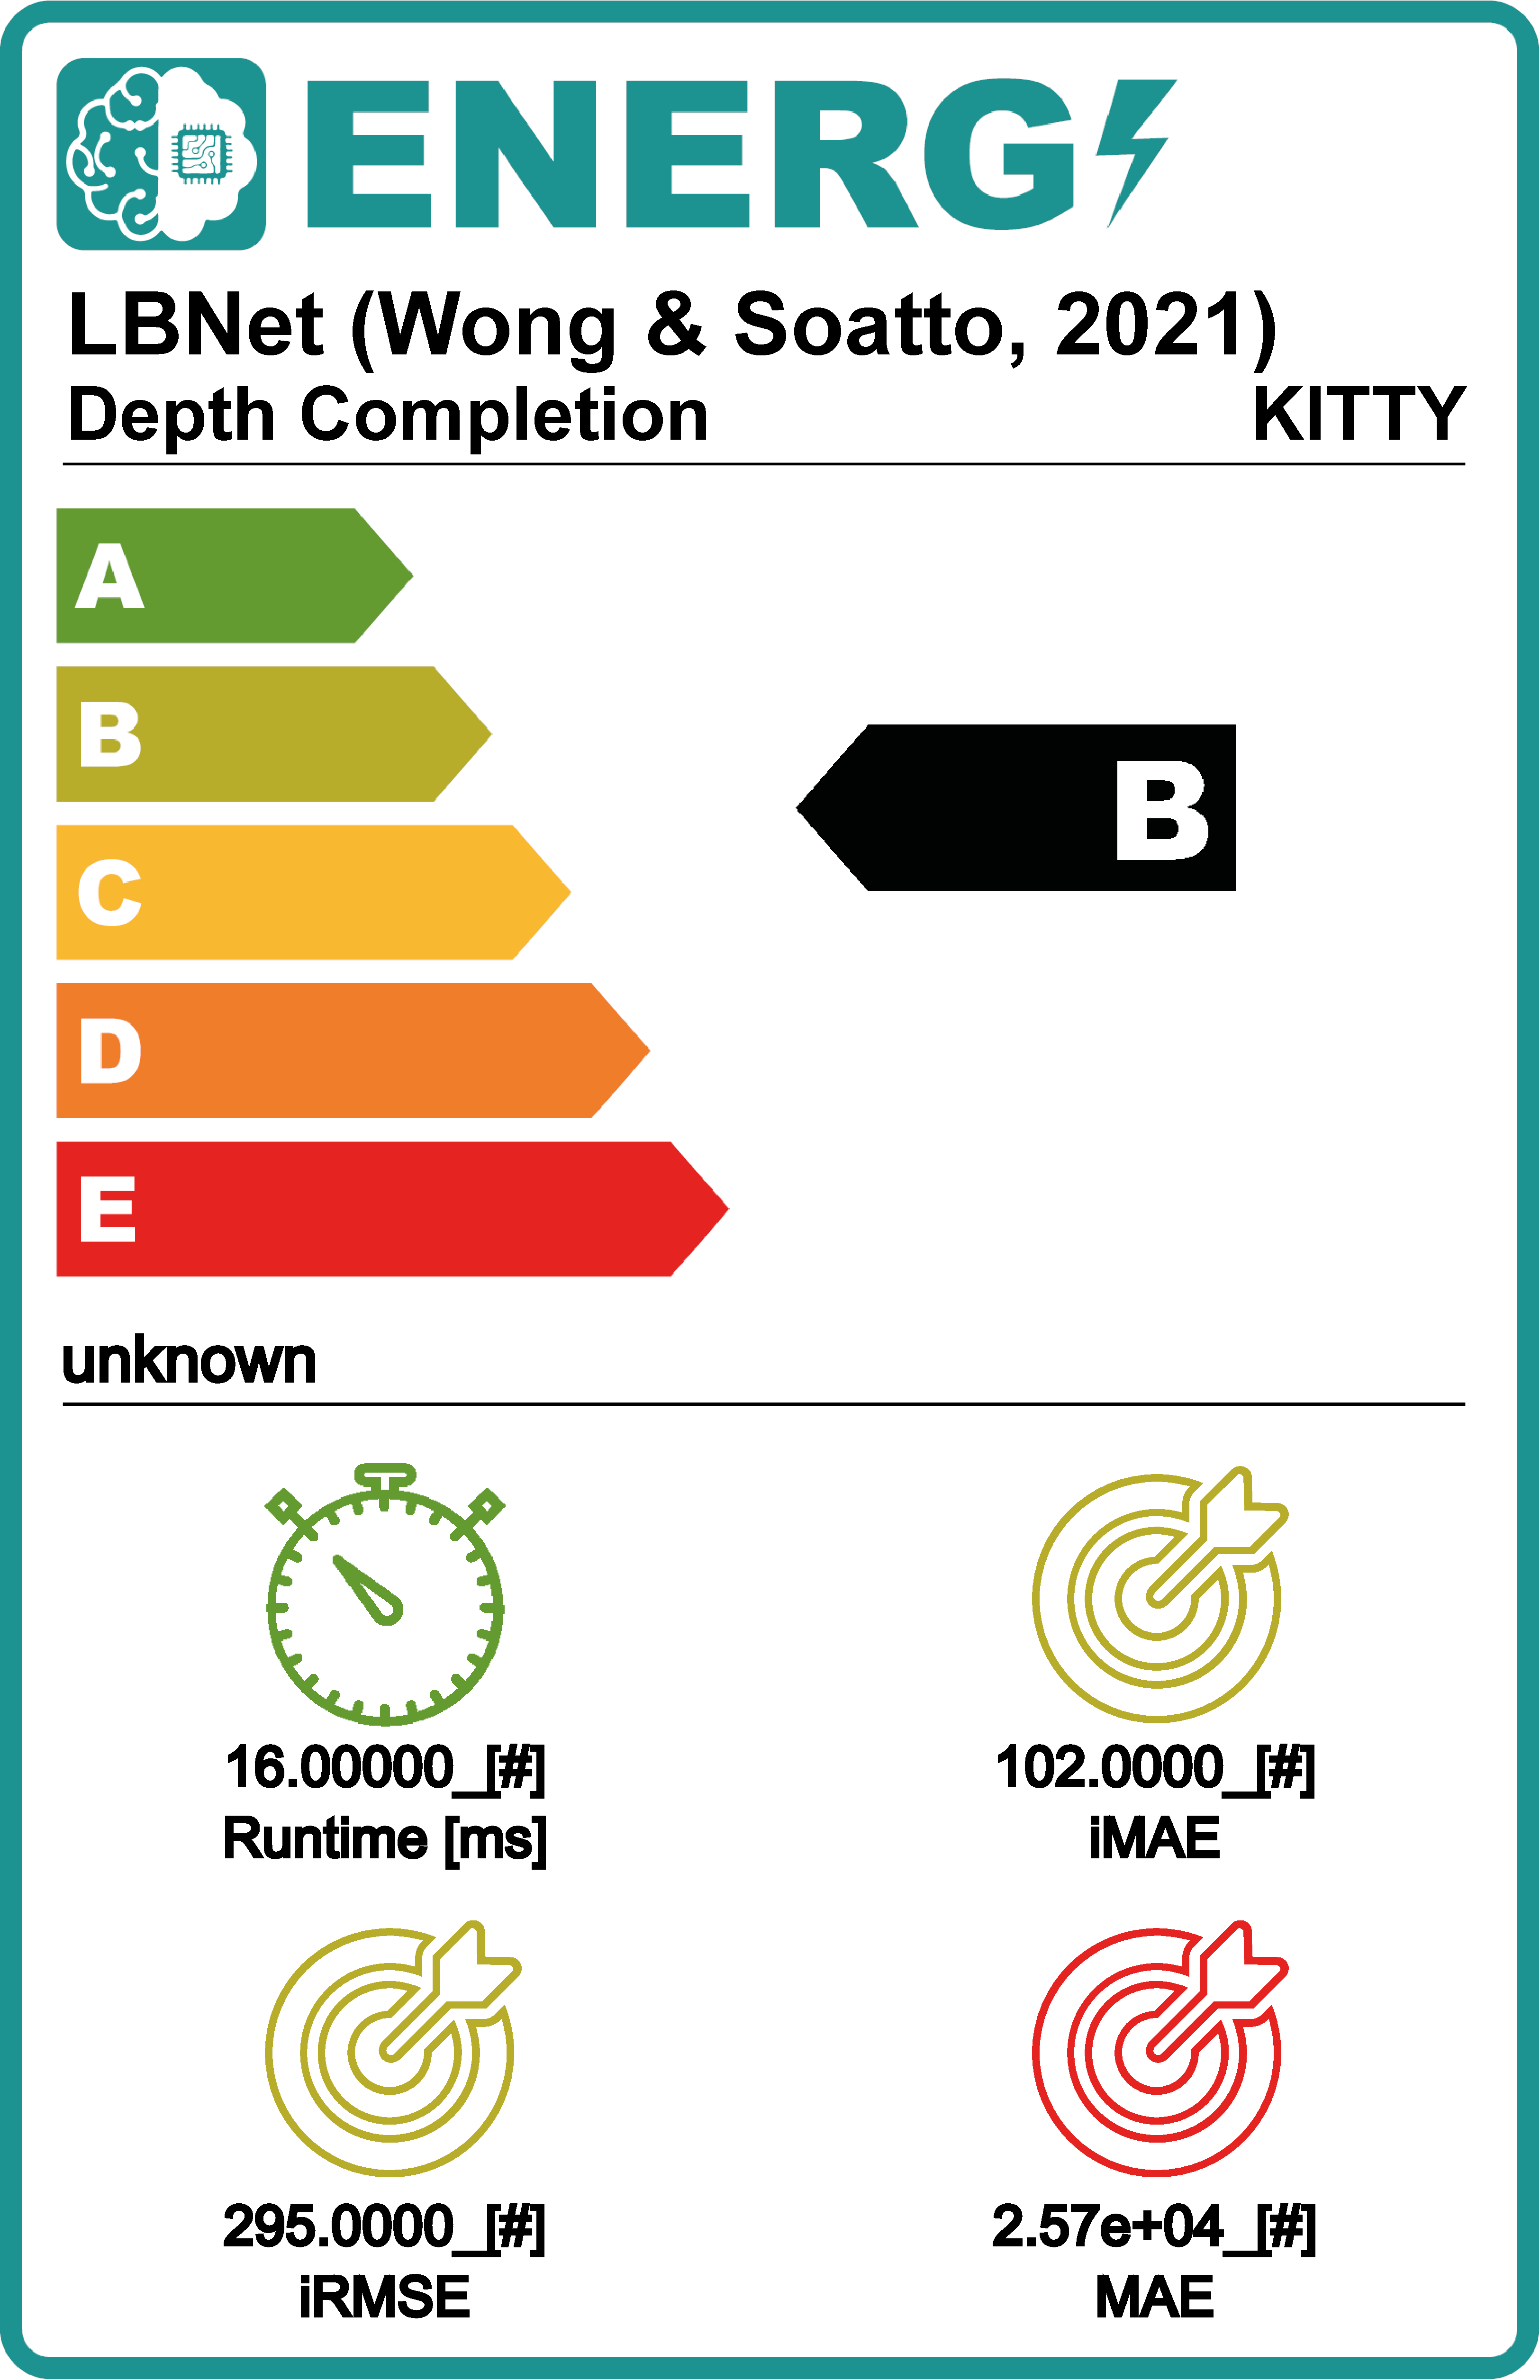
\includegraphics[width=.22\textwidth]{fig/energy_label_KBNet_from_unsupervised-depth-completion-with-calibrated_unknown.pdf}
    \hfill
    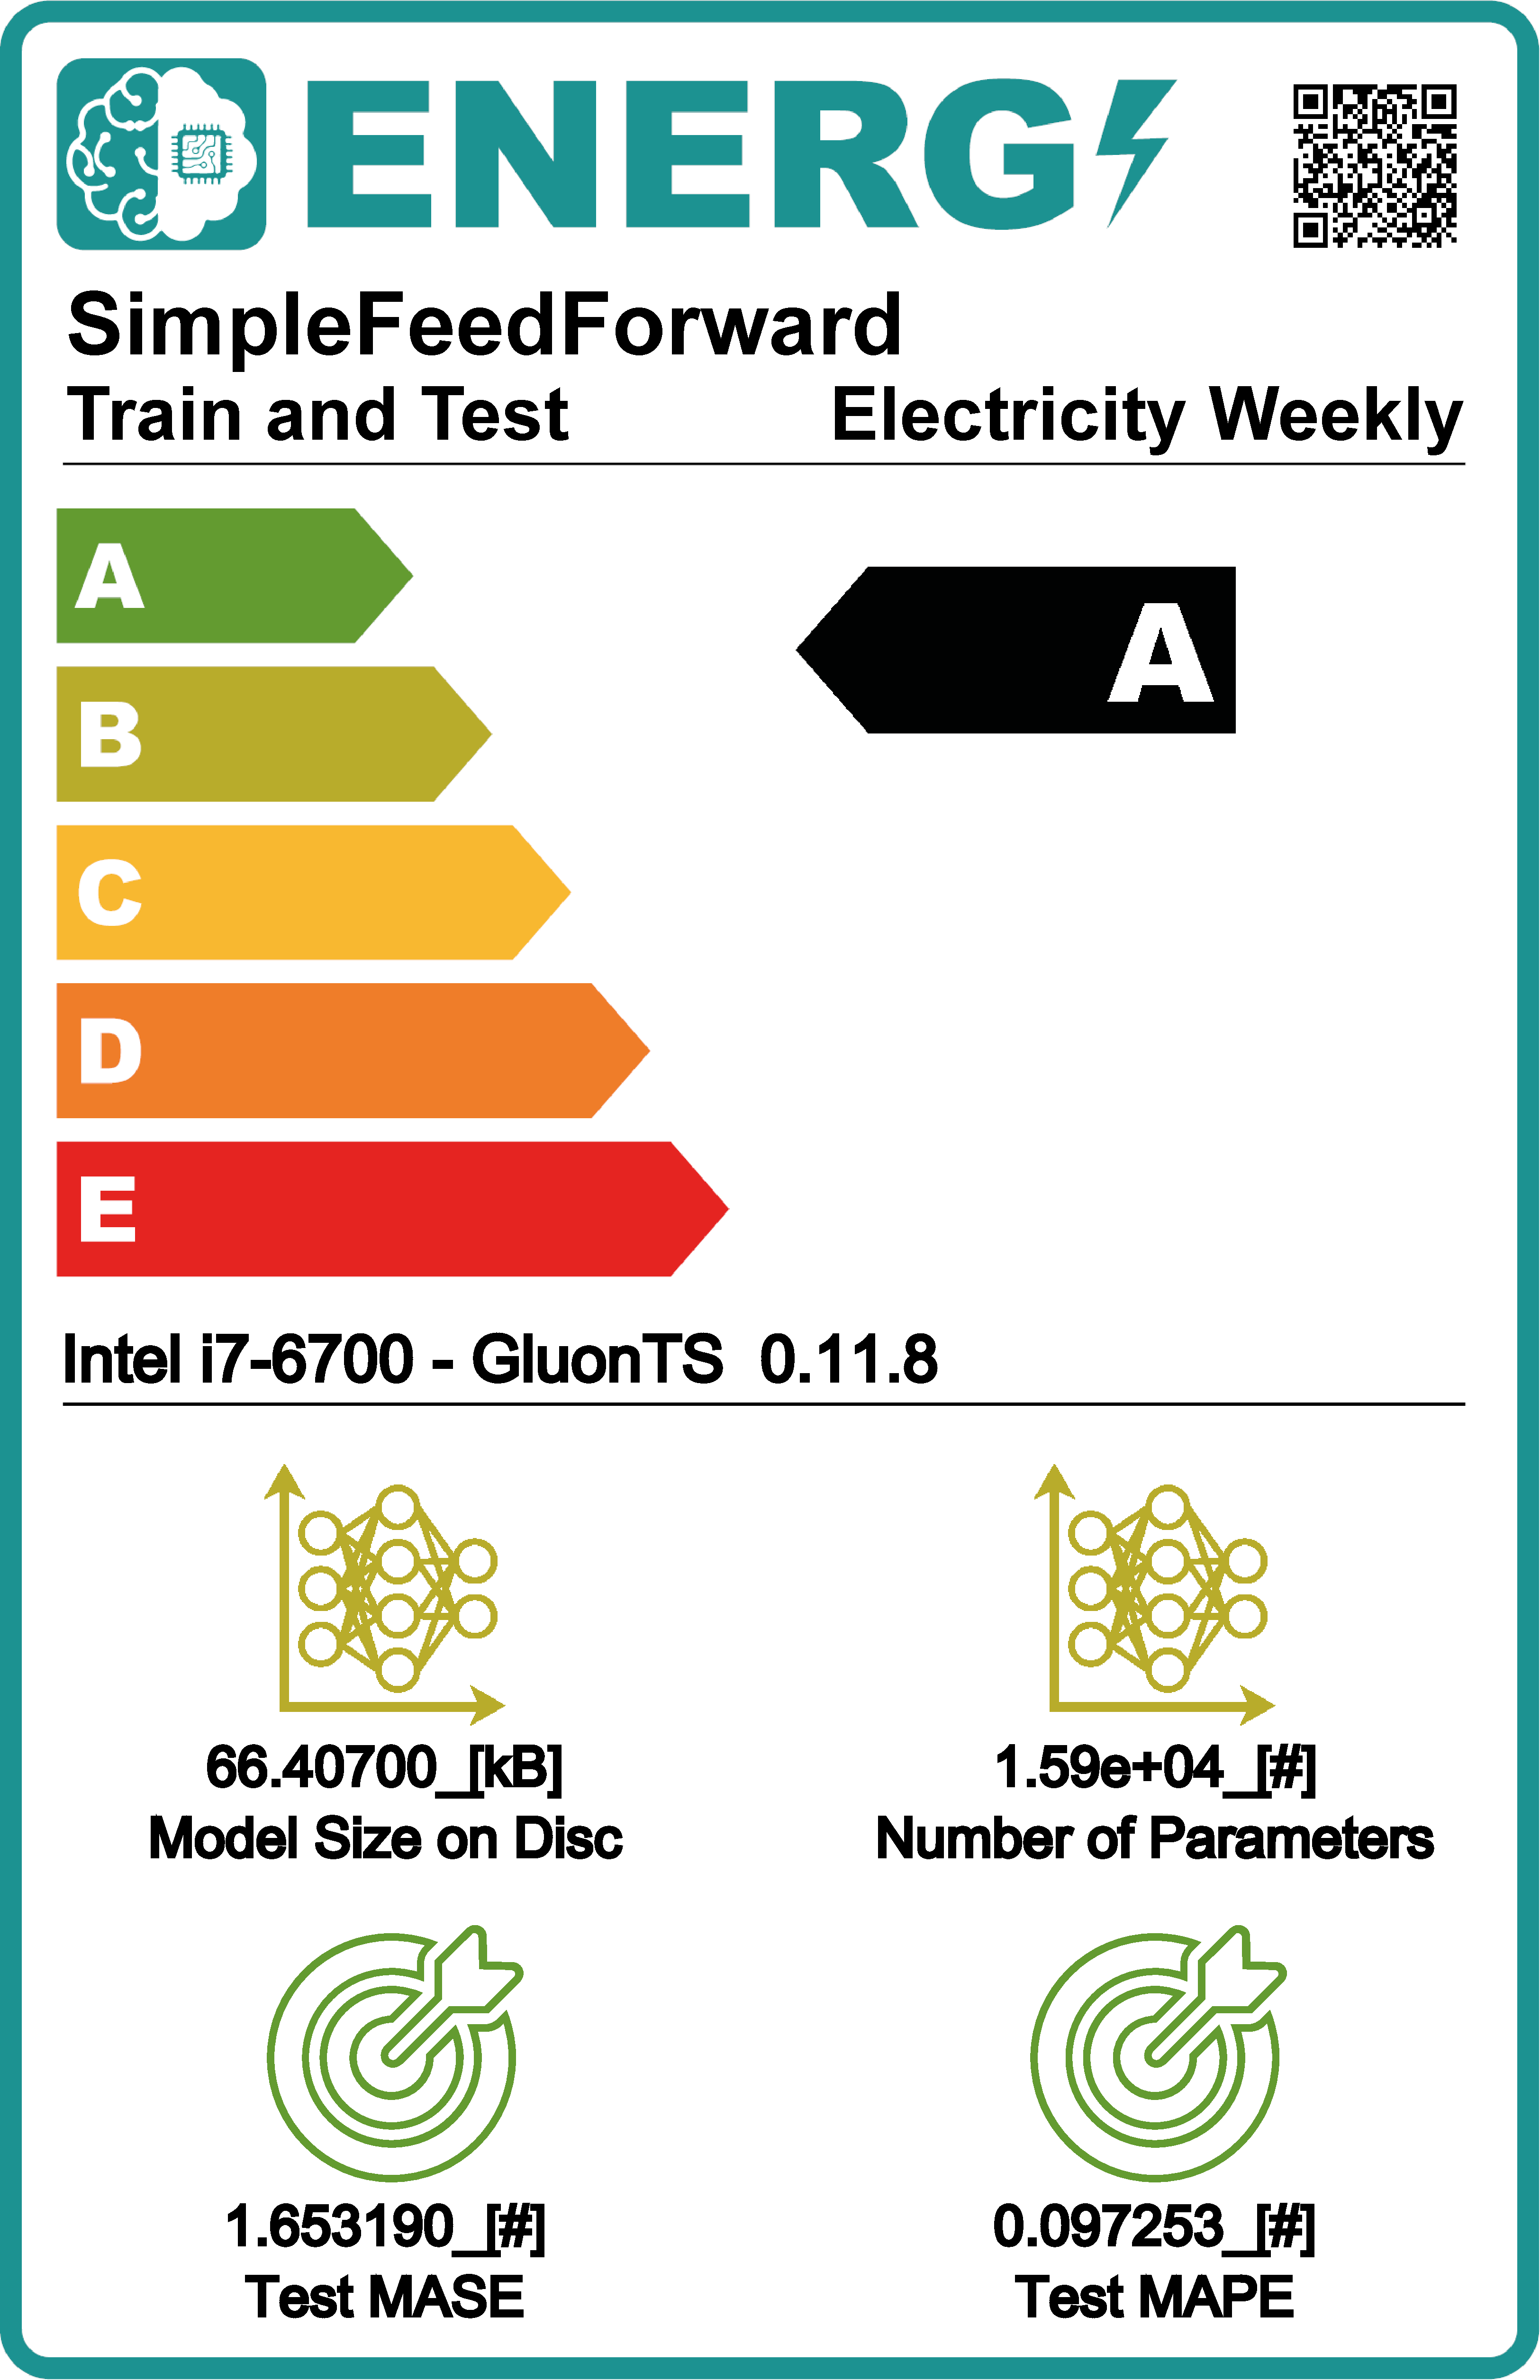
\includegraphics[width=.22\textwidth]{fig/energy_label_SimpleFeedForward_Intel_i7-6700_-_GluonTS__0.11.8.pdf}
    \caption{Exemplary property labels that convey information on method characteristics in a more comprehensible way. Colored badges indicate the relative positioning of real values with help from our index scaling approach. Trade-offs can be easily understood from this novel form of reporting.}
    \label{fig:labels}
\end{figure}

Lastly, let us consider how properties can be reported at higher level abstraction, to also inform users without fundamental ML knowledge.
For that, we implement our suggestions of \Cref{sec:meth:automated_labeling} and display prototypical labels as generated by STREP in \Cref{fig:labels}.
They are inspired by the EU energy labels \cite{eu-washingmachines} and display efficiency and robustness information for selected models and data.
The colored badges indicate the intuitive meaning behind each property in a more comprehensible way (e.g., battery for power draw, target circle for accuracy, stopwatch for running time).
For determining the rating colors, we used rating boundaries based on the 20\%, 40\%, 60\%, and 80\% quantiles of all scored values for the specific property -- the very same boundaries are also displayed as colored rectangles in \Cref{fig:prop_spaces}.
While boundaries and ratings were determined from the index values, the labels display the more intuitive real measurements and hide away the complexity of relative scaling.
In addition, they textually inform on evaluation and environment setting and feature a QR code with additional information material.
These labels demonstrate how intricate trade-offs between properties of any ML method can be communicated to less informed users of the reporting framework.





\section{Conclusion}

Practitioners that want to develop sustainable and trustworthy ML systems require elaborate reporting on the current SOTA in their specific application domain.
While many frameworks for publishing ML results exist, they also have certain drawbacks: they are overly focused on predictive capabilities, only offer limited means for interactive use, and inform on a very technical level that is hard to understand for non-experts.
In this work, we analyzed the current state of reporting and suggested novel means for improving it.
Our proposed STREP framework addresses (s)ustainability via index scaling and compound scoring, which enables resource-aware comparisons of methods even across multiple software and hardware.
We improve on (t)rustworthiness by allowing users to interactively control the importance of single method properties for the overall assessment.
In addition, our (rep)orting framework automatically generates high-level labels, which communicate intricate results to users without fundamental ML knowledge in a more comprehensible way.
We used STREP to practically investigate established report databases in terms of their resource-awareness, where we uncovered major biases towards predictive quality.
Our experimental evaluation also demonstrates the feasibility of our proposed ideas.
The implementation of STREP is publicly available and can be easily extended -- we invite fellow researchers to use it for exploring trade-offs occurring with methods in their own ML domains.
While we specifically focused this paper on characterizing the current state, proposing means to improve it, and testing our suggestions in practice, we also see much potential for future work.
Firstly, we will further investigate reproducibility aspects of current reporting and try to improve our framework along this direction.
In addition, we plan on evaluating the usability of different reporting frameworks and our labels representations via user studies.
We hope that our work is a helpful contribution for establishing a better reporting paradigm, which makes future ML application and methods more sustainable and trustworthy.


%%===========================================================================================%%
%% If you are submitting to one of the Nature Portfolio journals, using the eJP submission   %%
%% system, please include the references within the manuscript file itself. You may do this  %%
%% by copying the reference list from your .bbl file, paste it into the main manuscript .tex %%
%% file, and delete the associated \verb+\bibliography+ commands.                            %%
%%===========================================================================================%%

\bibliography{sn-bibliography}% common bib file
%% if required, the content of .bbl file can be included here once bbl is generated
%%\input sn-article.bbl


\end{document}
